\documentclass[twoside]{book}

% Packages required by doxygen
\usepackage{fixltx2e}
\usepackage{calc}
\usepackage{doxygen}
\usepackage[export]{adjustbox} % also loads graphicx
\usepackage{graphicx}
\usepackage[utf8]{inputenc}
\usepackage{makeidx}
\usepackage{multicol}
\usepackage{multirow}
\PassOptionsToPackage{warn}{textcomp}
\usepackage{textcomp}
\usepackage[nointegrals]{wasysym}
\usepackage[table]{xcolor}

% Font selection
\usepackage[T1]{fontenc}
\usepackage[scaled=.90]{helvet}
\usepackage{courier}
\usepackage{amssymb}
\usepackage{sectsty}
\renewcommand{\familydefault}{\sfdefault}
\allsectionsfont{%
  \fontseries{bc}\selectfont%
  \color{darkgray}%
}
\renewcommand{\DoxyLabelFont}{%
  \fontseries{bc}\selectfont%
  \color{darkgray}%
}
\newcommand{\+}{\discretionary{\mbox{\scriptsize$\hookleftarrow$}}{}{}}

% Page & text layout
\usepackage{geometry}
\geometry{%
  a4paper,%
  top=2.5cm,%
  bottom=2.5cm,%
  left=2.5cm,%
  right=2.5cm%
}
\tolerance=750
\hfuzz=15pt
\hbadness=750
\setlength{\emergencystretch}{15pt}
\setlength{\parindent}{0cm}
\setlength{\parskip}{3ex plus 2ex minus 2ex}
\makeatletter
\renewcommand{\paragraph}{%
  \@startsection{paragraph}{4}{0ex}{-1.0ex}{1.0ex}{%
    \normalfont\normalsize\bfseries\SS@parafont%
  }%
}
\renewcommand{\subparagraph}{%
  \@startsection{subparagraph}{5}{0ex}{-1.0ex}{1.0ex}{%
    \normalfont\normalsize\bfseries\SS@subparafont%
  }%
}
\makeatother

% Headers & footers
\usepackage{fancyhdr}
\pagestyle{fancyplain}
\fancyhead[LE]{\fancyplain{}{\bfseries\thepage}}
\fancyhead[CE]{\fancyplain{}{}}
\fancyhead[RE]{\fancyplain{}{\bfseries\leftmark}}
\fancyhead[LO]{\fancyplain{}{\bfseries\rightmark}}
\fancyhead[CO]{\fancyplain{}{}}
\fancyhead[RO]{\fancyplain{}{\bfseries\thepage}}
\fancyfoot[LE]{\fancyplain{}{}}
\fancyfoot[CE]{\fancyplain{}{}}
\fancyfoot[RE]{\fancyplain{}{\bfseries\scriptsize Generated by Doxygen }}
\fancyfoot[LO]{\fancyplain{}{\bfseries\scriptsize Generated by Doxygen }}
\fancyfoot[CO]{\fancyplain{}{}}
\fancyfoot[RO]{\fancyplain{}{}}
\renewcommand{\footrulewidth}{0.4pt}
\renewcommand{\chaptermark}[1]{%
  \markboth{#1}{}%
}
\renewcommand{\sectionmark}[1]{%
  \markright{\thesection\ #1}%
}

% Indices & bibliography
\usepackage{natbib}
\usepackage[titles]{tocloft}
\setcounter{tocdepth}{3}
\setcounter{secnumdepth}{5}
\makeindex

% Hyperlinks (required, but should be loaded last)
\usepackage{ifpdf}
\ifpdf
  \usepackage[pdftex,pagebackref=true]{hyperref}
\else
  \usepackage[ps2pdf,pagebackref=true]{hyperref}
\fi
\hypersetup{%
  colorlinks=true,%
  linkcolor=blue,%
  citecolor=blue,%
  unicode%
}

% Custom commands
\newcommand{\clearemptydoublepage}{%
  \newpage{\pagestyle{empty}\cleardoublepage}%
}

\usepackage{caption}
\captionsetup{labelsep=space,justification=centering,font={bf},singlelinecheck=off,skip=4pt,position=top}

%===== C O N T E N T S =====

\begin{document}

% Titlepage & ToC
\hypersetup{pageanchor=false,
             bookmarksnumbered=true,
             pdfencoding=unicode
            }
\pagenumbering{alph}
\begin{titlepage}
\vspace*{7cm}
\begin{center}%
{\Large lxm32 }\\
\vspace*{1cm}
{\large Generated by Doxygen 1.8.13}\\
\end{center}
\end{titlepage}
\clearemptydoublepage
\pagenumbering{roman}
\tableofcontents
\clearemptydoublepage
\pagenumbering{arabic}
\hypersetup{pageanchor=true}

%--- Begin generated contents ---
\chapter{L\+X\+M32}
\label{md__r_e_a_d_m_e}
\Hypertarget{md__r_e_a_d_m_e}
\input{md__r_e_a_d_m_e}
\chapter{Class Index}
\section{Class List}
Here are the classes, structs, unions and interfaces with brief descriptions\+:\begin{DoxyCompactList}
\item\contentsline{section}{\hyperlink{classc_joystick}{c\+Joystick} }{\pageref{classc_joystick}}{}
\item\contentsline{section}{\hyperlink{class_c_a_nopen_1_1_driver}{C\+A\+Nopen\+::\+Driver} }{\pageref{class_c_a_nopen_1_1_driver}}{}
\item\contentsline{section}{\hyperlink{structjoystick__position}{joystick\+\_\+position} }{\pageref{structjoystick__position}}{}
\item\contentsline{section}{\hyperlink{structjoystick__state}{joystick\+\_\+state} }{\pageref{structjoystick__state}}{}
\item\contentsline{section}{\hyperlink{class_c_a_nopen_1_1_l_x_m32}{C\+A\+Nopen\+::\+L\+X\+M32} }{\pageref{class_c_a_nopen_1_1_l_x_m32}}{}
\item\contentsline{section}{\hyperlink{class_c_a_nopen_1_1_message}{C\+A\+Nopen\+::\+Message} }{\pageref{class_c_a_nopen_1_1_message}}{}
\item\contentsline{section}{\hyperlink{class_c_a_nopen_1_1_n_m_t_message}{C\+A\+Nopen\+::\+N\+M\+T\+Message} }{\pageref{class_c_a_nopen_1_1_n_m_t_message}}{}
\item\contentsline{section}{\hyperlink{class_c_a_nopen_1_1_payload}{C\+A\+Nopen\+::\+Payload} }{\pageref{class_c_a_nopen_1_1_payload}}{}
\item\contentsline{section}{\hyperlink{class_c_a_nopen_1_1_p_d_o_message}{C\+A\+Nopen\+::\+P\+D\+O\+Message} }{\pageref{class_c_a_nopen_1_1_p_d_o_message}}{}
\item\contentsline{section}{\hyperlink{class_c_a_nopen_1_1_s_d_o_inbound}{C\+A\+Nopen\+::\+S\+D\+O\+Inbound} }{\pageref{class_c_a_nopen_1_1_s_d_o_inbound}}{}
\item\contentsline{section}{\hyperlink{class_c_a_nopen_1_1_s_d_o_message}{C\+A\+Nopen\+::\+S\+D\+O\+Message} }{\pageref{class_c_a_nopen_1_1_s_d_o_message}}{}
\item\contentsline{section}{\hyperlink{class_c_a_nopen_1_1_s_d_o_outbound}{C\+A\+Nopen\+::\+S\+D\+O\+Outbound} }{\pageref{class_c_a_nopen_1_1_s_d_o_outbound}}{}
\item\contentsline{section}{\hyperlink{class_c_a_nopen_1_1_s_d_o_outbound_read}{C\+A\+Nopen\+::\+S\+D\+O\+Outbound\+Read} }{\pageref{class_c_a_nopen_1_1_s_d_o_outbound_read}}{}
\item\contentsline{section}{\hyperlink{class_c_a_nopen_1_1_s_d_o_outbound_write}{C\+A\+Nopen\+::\+S\+D\+O\+Outbound\+Write} }{\pageref{class_c_a_nopen_1_1_s_d_o_outbound_write}}{}
\item\contentsline{section}{\hyperlink{class_c_a_nopen_1_1_socket}{C\+A\+Nopen\+::\+Socket} \\*Canopen object able to send command through a C\+AN interface using U\+N\+IX sockets }{\pageref{class_c_a_nopen_1_1_socket}}{}
\item\contentsline{section}{\hyperlink{structsss}{sss$<$ T $>$} }{\pageref{structsss}}{}
\end{DoxyCompactList}

\chapter{File Index}
\section{File List}
Here is a list of all files with brief descriptions\+:\begin{DoxyCompactList}
\item\contentsline{section}{/home/adev/\+Documents/\+S\+T\+E\+C\+H/lxm32/build/\+C\+Make\+Files/\hyperlink{feature__tests_8c}{feature\+\_\+tests.\+c} }{\pageref{feature__tests_8c}}{}
\item\contentsline{section}{/home/adev/\+Documents/\+S\+T\+E\+C\+H/lxm32/build/\+C\+Make\+Files/\hyperlink{feature__tests_8cxx}{feature\+\_\+tests.\+cxx} }{\pageref{feature__tests_8cxx}}{}
\item\contentsline{section}{/home/adev/\+Documents/\+S\+T\+E\+C\+H/lxm32/build/\+C\+Make\+Files/3.\+10.\+2/\+Compiler\+Id\+C/\hyperlink{_c_make_c_compiler_id_8c}{C\+Make\+C\+Compiler\+Id.\+c} }{\pageref{_c_make_c_compiler_id_8c}}{}
\item\contentsline{section}{/home/adev/\+Documents/\+S\+T\+E\+C\+H/lxm32/build/\+C\+Make\+Files/3.\+10.\+2/\+Compiler\+Id\+C\+X\+X/\hyperlink{_c_make_c_x_x_compiler_id_8cpp}{C\+Make\+C\+X\+X\+Compiler\+Id.\+cpp} }{\pageref{_c_make_c_x_x_compiler_id_8cpp}}{}
\item\contentsline{section}{/home/adev/\+Documents/\+S\+T\+E\+C\+H/lxm32/include/\hyperlink{_c_a_ndriver_8h}{C\+A\+Ndriver.\+h} }{\pageref{_c_a_ndriver_8h}}{}
\item\contentsline{section}{/home/adev/\+Documents/\+S\+T\+E\+C\+H/lxm32/include/\hyperlink{_c_a_nopen__driver_8h}{C\+A\+Nopen\+\_\+driver.\+h} }{\pageref{_c_a_nopen__driver_8h}}{}
\item\contentsline{section}{/home/adev/\+Documents/\+S\+T\+E\+C\+H/lxm32/include/\hyperlink{_c_a_nopen__lxm32_8h}{C\+A\+Nopen\+\_\+lxm32.\+h} }{\pageref{_c_a_nopen__lxm32_8h}}{}
\item\contentsline{section}{/home/adev/\+Documents/\+S\+T\+E\+C\+H/lxm32/lib/canopen/include/\hyperlink{_c_a_nopen__socket_8h}{C\+A\+Nopen\+\_\+socket.\+h} \\*Canopen object able to send command through a C\+AN interface using the U\+N\+IX socket }{\pageref{_c_a_nopen__socket_8h}}{}
\item\contentsline{section}{/home/adev/\+Documents/\+S\+T\+E\+C\+H/lxm32/lib/canopen/include/\hyperlink{config_8h}{config.\+h} }{\pageref{config_8h}}{}
\item\contentsline{section}{/home/adev/\+Documents/\+S\+T\+E\+C\+H/lxm32/lib/canopen/include/\hyperlink{message_8h}{message.\+h} }{\pageref{message_8h}}{}
\item\contentsline{section}{/home/adev/\+Documents/\+S\+T\+E\+C\+H/lxm32/lib/canopen/include/\hyperlink{nmt_8h}{nmt.\+h} }{\pageref{nmt_8h}}{}
\item\contentsline{section}{/home/adev/\+Documents/\+S\+T\+E\+C\+H/lxm32/lib/canopen/include/\hyperlink{payload_8h}{payload.\+h} }{\pageref{payload_8h}}{}
\item\contentsline{section}{/home/adev/\+Documents/\+S\+T\+E\+C\+H/lxm32/lib/canopen/include/\hyperlink{pdo_8h}{pdo.\+h} }{\pageref{pdo_8h}}{}
\item\contentsline{section}{/home/adev/\+Documents/\+S\+T\+E\+C\+H/lxm32/lib/canopen/include/\hyperlink{sdo_8h}{sdo.\+h} }{\pageref{sdo_8h}}{}
\item\contentsline{section}{/home/adev/\+Documents/\+S\+T\+E\+C\+H/lxm32/lib/canopen/src/\hyperlink{_c_a_nopen__socket_8cpp}{C\+A\+Nopen\+\_\+socket.\+cpp} }{\pageref{_c_a_nopen__socket_8cpp}}{}
\item\contentsline{section}{/home/adev/\+Documents/\+S\+T\+E\+C\+H/lxm32/lib/canopen/src/\hyperlink{lib_2canopen_2src_2main_8cpp}{main.\+cpp} }{\pageref{lib_2canopen_2src_2main_8cpp}}{}
\item\contentsline{section}{/home/adev/\+Documents/\+S\+T\+E\+C\+H/lxm32/lib/canopen/src/\hyperlink{message_8cpp}{message.\+cpp} }{\pageref{message_8cpp}}{}
\item\contentsline{section}{/home/adev/\+Documents/\+S\+T\+E\+C\+H/lxm32/lib/canopen/src/\hyperlink{nmt_8cpp}{nmt.\+cpp} }{\pageref{nmt_8cpp}}{}
\item\contentsline{section}{/home/adev/\+Documents/\+S\+T\+E\+C\+H/lxm32/lib/canopen/src/\hyperlink{payload_8cpp}{payload.\+cpp} }{\pageref{payload_8cpp}}{}
\item\contentsline{section}{/home/adev/\+Documents/\+S\+T\+E\+C\+H/lxm32/lib/canopen/src/\hyperlink{pdo_8cpp}{pdo.\+cpp} }{\pageref{pdo_8cpp}}{}
\item\contentsline{section}{/home/adev/\+Documents/\+S\+T\+E\+C\+H/lxm32/lib/canopen/src/\hyperlink{sdo_8cpp}{sdo.\+cpp} }{\pageref{sdo_8cpp}}{}
\item\contentsline{section}{/home/adev/\+Documents/\+S\+T\+E\+C\+H/lxm32/lib/joystick/include/\hyperlink{joystick_8h}{joystick.\+h} }{\pageref{joystick_8h}}{}
\item\contentsline{section}{/home/adev/\+Documents/\+S\+T\+E\+C\+H/lxm32/lib/joystick/src/\hyperlink{joystick_8cpp}{joystick.\+cpp} }{\pageref{joystick_8cpp}}{}
\item\contentsline{section}{/home/adev/\+Documents/\+S\+T\+E\+C\+H/lxm32/lib/joystick/src/\hyperlink{lib_2joystick_2src_2main_8cpp}{main.\+cpp} }{\pageref{lib_2joystick_2src_2main_8cpp}}{}
\item\contentsline{section}{/home/adev/\+Documents/\+S\+T\+E\+C\+H/lxm32/src/\hyperlink{_c_a_nopen__driver_8cpp}{C\+A\+Nopen\+\_\+driver.\+cpp} }{\pageref{_c_a_nopen__driver_8cpp}}{}
\item\contentsline{section}{/home/adev/\+Documents/\+S\+T\+E\+C\+H/lxm32/src/\hyperlink{_c_a_nopen__lxm32_8cpp}{C\+A\+Nopen\+\_\+lxm32.\+cpp} }{\pageref{_c_a_nopen__lxm32_8cpp}}{}
\item\contentsline{section}{/home/adev/\+Documents/\+S\+T\+E\+C\+H/lxm32/src/\hyperlink{src_2main_8cpp}{main.\+cpp} }{\pageref{src_2main_8cpp}}{}
\end{DoxyCompactList}

\chapter{Class Documentation}
\hypertarget{class_l_x_m32}{}\section{L\+X\+M32 Class Reference}
\label{class_l_x_m32}\index{L\+X\+M32@{L\+X\+M32}}


{\ttfamily \#include $<$Lexium32\+A\+\_\+canopen.\+h$>$}

\subsection*{Public Member Functions}
\begin{DoxyCompactItemize}
\item 
\hyperlink{class_l_x_m32_aa4a3e84b72c79b4d47e9f842a8977f98}{L\+X\+M32} (const char $\ast$ifname, uint16\+\_\+t can\+\_\+id, bool verbose=false)
\item 
void \hyperlink{class_l_x_m32_a3d325b9b19432dc05240ccfc328363d9}{init} ()
\item 
void \hyperlink{class_l_x_m32_a53198cf491d6b00d698bac5a55bbe5d4}{start} ()
\item 
void \hyperlink{class_l_x_m32_a73364111a5c2be2d60b7456704f7b9a8}{stop} ()
\item 
void \hyperlink{class_l_x_m32_a3b470e3d484fc0fb2a208df10a8e29e7}{new\+\_\+pos} (int32\+\_\+t pos)
\item 
void \hyperlink{class_l_x_m32_a4087402e009dd3be18765caac410d412}{set\+\_\+mode} (int8\+\_\+t mode)
\item 
void \hyperlink{class_l_x_m32_aa36cd9154a11f3388715fa2f482c37ca}{get\+\_\+param} ()
\item 
void \hyperlink{class_l_x_m32_a201d8f9da28994a92612e2618b7a1167}{print\+\_\+status} ()
\item 
void \hyperlink{class_l_x_m32_a545b23fab3528a8039bb2cc62808f9f5}{print\+\_\+control} ()
\end{DoxyCompactItemize}


\subsection{Detailed Description}


Definition at line 43 of file Lexium32\+A\+\_\+canopen.\+h.



\subsection{Constructor \& Destructor Documentation}
\mbox{\Hypertarget{class_l_x_m32_aa4a3e84b72c79b4d47e9f842a8977f98}\label{class_l_x_m32_aa4a3e84b72c79b4d47e9f842a8977f98}} 
\index{L\+X\+M32@{L\+X\+M32}!L\+X\+M32@{L\+X\+M32}}
\index{L\+X\+M32@{L\+X\+M32}!L\+X\+M32@{L\+X\+M32}}
\subsubsection{\texorpdfstring{L\+X\+M32()}{LXM32()}}
{\footnotesize\ttfamily L\+X\+M32\+::\+L\+X\+M32 (\begin{DoxyParamCaption}\item[{const char $\ast$}]{ifname,  }\item[{uint16\+\_\+t}]{can\+\_\+id,  }\item[{bool}]{verbose = {\ttfamily false} }\end{DoxyParamCaption})\hspace{0.3cm}{\ttfamily [inline]}}



Definition at line 46 of file Lexium32\+A\+\_\+canopen.\+h.



\subsection{Member Function Documentation}
\mbox{\Hypertarget{class_l_x_m32_aa36cd9154a11f3388715fa2f482c37ca}\label{class_l_x_m32_aa36cd9154a11f3388715fa2f482c37ca}} 
\index{L\+X\+M32@{L\+X\+M32}!get\+\_\+param@{get\+\_\+param}}
\index{get\+\_\+param@{get\+\_\+param}!L\+X\+M32@{L\+X\+M32}}
\subsubsection{\texorpdfstring{get\+\_\+param()}{get\_param()}}
{\footnotesize\ttfamily void L\+X\+M32\+::get\+\_\+param (\begin{DoxyParamCaption}{ }\end{DoxyParamCaption})\hspace{0.3cm}{\ttfamily [inline]}}



Definition at line 137 of file Lexium32\+A\+\_\+canopen.\+h.

\mbox{\Hypertarget{class_l_x_m32_a3d325b9b19432dc05240ccfc328363d9}\label{class_l_x_m32_a3d325b9b19432dc05240ccfc328363d9}} 
\index{L\+X\+M32@{L\+X\+M32}!init@{init}}
\index{init@{init}!L\+X\+M32@{L\+X\+M32}}
\subsubsection{\texorpdfstring{init()}{init()}}
{\footnotesize\ttfamily void L\+X\+M32\+::init (\begin{DoxyParamCaption}{ }\end{DoxyParamCaption})\hspace{0.3cm}{\ttfamily [inline]}}



Definition at line 67 of file Lexium32\+A\+\_\+canopen.\+h.

\mbox{\Hypertarget{class_l_x_m32_a3b470e3d484fc0fb2a208df10a8e29e7}\label{class_l_x_m32_a3b470e3d484fc0fb2a208df10a8e29e7}} 
\index{L\+X\+M32@{L\+X\+M32}!new\+\_\+pos@{new\+\_\+pos}}
\index{new\+\_\+pos@{new\+\_\+pos}!L\+X\+M32@{L\+X\+M32}}
\subsubsection{\texorpdfstring{new\+\_\+pos()}{new\_pos()}}
{\footnotesize\ttfamily void L\+X\+M32\+::new\+\_\+pos (\begin{DoxyParamCaption}\item[{int32\+\_\+t}]{pos }\end{DoxyParamCaption})\hspace{0.3cm}{\ttfamily [inline]}}



Definition at line 115 of file Lexium32\+A\+\_\+canopen.\+h.

\mbox{\Hypertarget{class_l_x_m32_a545b23fab3528a8039bb2cc62808f9f5}\label{class_l_x_m32_a545b23fab3528a8039bb2cc62808f9f5}} 
\index{L\+X\+M32@{L\+X\+M32}!print\+\_\+control@{print\+\_\+control}}
\index{print\+\_\+control@{print\+\_\+control}!L\+X\+M32@{L\+X\+M32}}
\subsubsection{\texorpdfstring{print\+\_\+control()}{print\_control()}}
{\footnotesize\ttfamily void L\+X\+M32\+::print\+\_\+control (\begin{DoxyParamCaption}{ }\end{DoxyParamCaption})\hspace{0.3cm}{\ttfamily [inline]}}



Definition at line 191 of file Lexium32\+A\+\_\+canopen.\+h.

\mbox{\Hypertarget{class_l_x_m32_a201d8f9da28994a92612e2618b7a1167}\label{class_l_x_m32_a201d8f9da28994a92612e2618b7a1167}} 
\index{L\+X\+M32@{L\+X\+M32}!print\+\_\+status@{print\+\_\+status}}
\index{print\+\_\+status@{print\+\_\+status}!L\+X\+M32@{L\+X\+M32}}
\subsubsection{\texorpdfstring{print\+\_\+status()}{print\_status()}}
{\footnotesize\ttfamily void L\+X\+M32\+::print\+\_\+status (\begin{DoxyParamCaption}{ }\end{DoxyParamCaption})\hspace{0.3cm}{\ttfamily [inline]}}



Definition at line 143 of file Lexium32\+A\+\_\+canopen.\+h.

\mbox{\Hypertarget{class_l_x_m32_a4087402e009dd3be18765caac410d412}\label{class_l_x_m32_a4087402e009dd3be18765caac410d412}} 
\index{L\+X\+M32@{L\+X\+M32}!set\+\_\+mode@{set\+\_\+mode}}
\index{set\+\_\+mode@{set\+\_\+mode}!L\+X\+M32@{L\+X\+M32}}
\subsubsection{\texorpdfstring{set\+\_\+mode()}{set\_mode()}}
{\footnotesize\ttfamily void L\+X\+M32\+::set\+\_\+mode (\begin{DoxyParamCaption}\item[{int8\+\_\+t}]{mode }\end{DoxyParamCaption})\hspace{0.3cm}{\ttfamily [inline]}}



Definition at line 127 of file Lexium32\+A\+\_\+canopen.\+h.

\mbox{\Hypertarget{class_l_x_m32_a53198cf491d6b00d698bac5a55bbe5d4}\label{class_l_x_m32_a53198cf491d6b00d698bac5a55bbe5d4}} 
\index{L\+X\+M32@{L\+X\+M32}!start@{start}}
\index{start@{start}!L\+X\+M32@{L\+X\+M32}}
\subsubsection{\texorpdfstring{start()}{start()}}
{\footnotesize\ttfamily void L\+X\+M32\+::start (\begin{DoxyParamCaption}{ }\end{DoxyParamCaption})\hspace{0.3cm}{\ttfamily [inline]}}



Definition at line 92 of file Lexium32\+A\+\_\+canopen.\+h.

\mbox{\Hypertarget{class_l_x_m32_a73364111a5c2be2d60b7456704f7b9a8}\label{class_l_x_m32_a73364111a5c2be2d60b7456704f7b9a8}} 
\index{L\+X\+M32@{L\+X\+M32}!stop@{stop}}
\index{stop@{stop}!L\+X\+M32@{L\+X\+M32}}
\subsubsection{\texorpdfstring{stop()}{stop()}}
{\footnotesize\ttfamily void L\+X\+M32\+::stop (\begin{DoxyParamCaption}{ }\end{DoxyParamCaption})\hspace{0.3cm}{\ttfamily [inline]}}



Definition at line 110 of file Lexium32\+A\+\_\+canopen.\+h.



The documentation for this class was generated from the following file\+:\begin{DoxyCompactItemize}
\item 
include/\hyperlink{_lexium32_a__canopen_8h}{Lexium32\+A\+\_\+canopen.\+h}\end{DoxyCompactItemize}

\chapter{File Documentation}
\hypertarget{_lexium32_a__canopen_8h}{}\section{include/\+Lexium32\+A\+\_\+canopen.h File Reference}
\label{_lexium32_a__canopen_8h}\index{include/\+Lexium32\+A\+\_\+canopen.\+h@{include/\+Lexium32\+A\+\_\+canopen.\+h}}
{\ttfamily \#include \char`\"{}canopen\+\_\+socket.\+h\char`\"{}}\newline
{\ttfamily \#include $<$string$>$}\newline
{\ttfamily \#include $<$unistd.\+h$>$}\newline
Include dependency graph for Lexium32\+A\+\_\+canopen.\+h\+:
\nopagebreak
\begin{figure}[H]
\begin{center}
\leavevmode
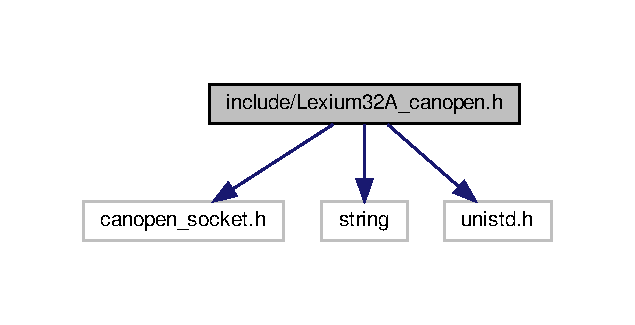
\includegraphics[width=305pt]{_lexium32_a__canopen_8h__incl}
\end{center}
\end{figure}
This graph shows which files directly or indirectly include this file\+:
\nopagebreak
\begin{figure}[H]
\begin{center}
\leavevmode
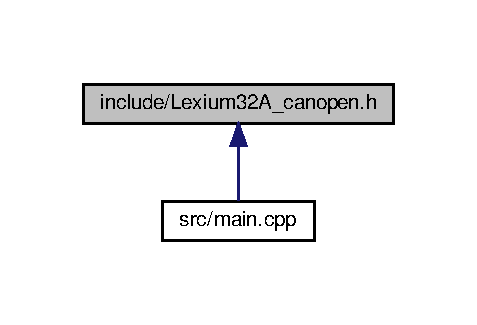
\includegraphics[width=229pt]{_lexium32_a__canopen_8h__dep__incl}
\end{center}
\end{figure}
\subsection*{Classes}
\begin{DoxyCompactItemize}
\item 
class \hyperlink{class_l_x_m32}{L\+X\+M32}
\end{DoxyCompactItemize}
\subsection*{Macros}
\begin{DoxyCompactItemize}
\item 
\#define \hyperlink{_lexium32_a__canopen_8h_a288301cb406c37bce2e676a61a47069f}{R\+E\+G\+\_\+\+C\+A\+Naddress}~0x30410002
\item 
\#define \hyperlink{_lexium32_a__canopen_8h_a0cc1502471745a5a5d2953588405e4bb}{R\+E\+G\+\_\+\+C\+A\+Nbaud}~0x30410003
\item 
\#define \hyperlink{_lexium32_a__canopen_8h_a45fd1c3357c3e7820e73914b4aa2d3ee}{R\+E\+G\+\_\+\+\_\+\+D\+C\+O\+Mstatus}~0x60410000
\item 
\#define \hyperlink{_lexium32_a__canopen_8h_adb964aa4eaba974ed438fee7b9d09ccd}{R\+E\+G\+\_\+\+D\+C\+O\+Mopmode}~0x60600000
\item 
\#define \hyperlink{_lexium32_a__canopen_8h_a37233bac366559f38558d6ffeb5daf01}{R\+E\+G\+\_\+\+D\+C\+O\+Mcontrol}~0x60400000
\item 
\#define \hyperlink{_lexium32_a__canopen_8h_ac2ea552341a2aacf207cfc8c8bcc27af}{R\+E\+G\+\_\+\+P\+Pp\+\_\+target}~0x607\+A0000
\item 
\#define \hyperlink{_lexium32_a__canopen_8h_a5684fffd76d166871a0f7618cb33fa76}{R\+E\+G\+\_\+\+P\+Pv\+\_\+target}~0x60810000
\item 
\#define \hyperlink{_lexium32_a__canopen_8h_aac1fb3a95430fb03df0455a3e849d076}{R\+E\+G\+\_\+\+P\+Poption}~0x60\+F20000
\item 
\#define \hyperlink{_lexium32_a__canopen_8h_ab2aeca9392d3d3fe2889e2a4799e53a4}{R\+E\+G\+\_\+\+J\+O\+Gactivate}~0x301\+B0009
\item 
\#define \hyperlink{_lexium32_a__canopen_8h_abd03ed23facc5aa2eac935fa69608547}{M\+O\+D\+E\+\_\+\+Profile\+Position}~1
\item 
\#define \hyperlink{_lexium32_a__canopen_8h_a73172a8fb87a3183ff29444335ba4fdb}{P\+Pctrl\+\_\+\+S\+E\+T\+\_\+\+P\+O\+I\+NT}~0x0010
\item 
\#define \hyperlink{_lexium32_a__canopen_8h_a88648c72edc2879a93ba4723ae3652e7}{P\+Pctrl\+\_\+\+O\+N\+\_\+\+T\+A\+R\+G\+ET}~0x0040
\item 
\#define \hyperlink{_lexium32_a__canopen_8h_ab9cafb4211b0fa97cfc73b15d7b72b11}{P\+Pctrl\+\_\+\+O\+N\+\_\+\+D\+I\+R\+E\+CT}~0x0020
\item 
\#define \hyperlink{_lexium32_a__canopen_8h_a0349d409f0d302bb5374bcd5cd77c126}{P\+Pctrl\+\_\+\+R\+E\+L\+A\+T\+I\+VE}~0x0040
\item 
\#define \hyperlink{_lexium32_a__canopen_8h_ac8368603aa9e8065efb0a231bd007ee5}{P\+Pctrl\+\_\+\+A\+B\+S\+O\+L\+U\+TE}~0x0000
\item 
\#define \hyperlink{_lexium32_a__canopen_8h_ac4772c1c1c24a4b5837a2000c62aa0a3}{O\+P\+\_\+\+S\+H\+U\+T\+D\+O\+WN}~0x0006
\item 
\#define \hyperlink{_lexium32_a__canopen_8h_acf9b640777e01c586865a1b2791fc8b9}{O\+P\+\_\+\+S\+W\+I\+T\+C\+H\+ON}~0x0007
\item 
\#define \hyperlink{_lexium32_a__canopen_8h_a05d94d73527d10913d800850b4ea65f4}{O\+P\+\_\+\+D\+I\+S\+A\+B\+L\+E\+V\+OL}~0x0000
\item 
\#define \hyperlink{_lexium32_a__canopen_8h_ac3cecf02598899083372e24e0093544c}{O\+P\+\_\+\+Q\+U\+I\+C\+K\+S\+T\+OP}~0x0002
\item 
\#define \hyperlink{_lexium32_a__canopen_8h_ad45ed0f1fc61ec91eea44c1e64daac17}{O\+P\+\_\+\+D\+I\+S\+A\+B\+L\+E\+OP}~0x0007
\item 
\#define \hyperlink{_lexium32_a__canopen_8h_ac2d32ebfb52f2cf10d7fec601f266a0f}{O\+P\+\_\+\+E\+N\+A\+B\+L\+E\+OP}~0x000F
\item 
\#define \hyperlink{_lexium32_a__canopen_8h_a64e5209a86a8aa06bd3e71c354616b1c}{O\+P\+\_\+\+F\+A\+U\+L\+T\+R\+E\+S\+E\+ST}~0x0080
\end{DoxyCompactItemize}


\subsection{Macro Definition Documentation}
\mbox{\Hypertarget{_lexium32_a__canopen_8h_abd03ed23facc5aa2eac935fa69608547}\label{_lexium32_a__canopen_8h_abd03ed23facc5aa2eac935fa69608547}} 
\index{Lexium32\+A\+\_\+canopen.\+h@{Lexium32\+A\+\_\+canopen.\+h}!M\+O\+D\+E\+\_\+\+Profile\+Position@{M\+O\+D\+E\+\_\+\+Profile\+Position}}
\index{M\+O\+D\+E\+\_\+\+Profile\+Position@{M\+O\+D\+E\+\_\+\+Profile\+Position}!Lexium32\+A\+\_\+canopen.\+h@{Lexium32\+A\+\_\+canopen.\+h}}
\subsubsection{\texorpdfstring{M\+O\+D\+E\+\_\+\+Profile\+Position}{MODE\_ProfilePosition}}
{\footnotesize\ttfamily \#define M\+O\+D\+E\+\_\+\+Profile\+Position~1}



Definition at line 24 of file Lexium32\+A\+\_\+canopen.\+h.

\mbox{\Hypertarget{_lexium32_a__canopen_8h_ad45ed0f1fc61ec91eea44c1e64daac17}\label{_lexium32_a__canopen_8h_ad45ed0f1fc61ec91eea44c1e64daac17}} 
\index{Lexium32\+A\+\_\+canopen.\+h@{Lexium32\+A\+\_\+canopen.\+h}!O\+P\+\_\+\+D\+I\+S\+A\+B\+L\+E\+OP@{O\+P\+\_\+\+D\+I\+S\+A\+B\+L\+E\+OP}}
\index{O\+P\+\_\+\+D\+I\+S\+A\+B\+L\+E\+OP@{O\+P\+\_\+\+D\+I\+S\+A\+B\+L\+E\+OP}!Lexium32\+A\+\_\+canopen.\+h@{Lexium32\+A\+\_\+canopen.\+h}}
\subsubsection{\texorpdfstring{O\+P\+\_\+\+D\+I\+S\+A\+B\+L\+E\+OP}{OP\_DISABLEOP}}
{\footnotesize\ttfamily \#define O\+P\+\_\+\+D\+I\+S\+A\+B\+L\+E\+OP~0x0007}



Definition at line 35 of file Lexium32\+A\+\_\+canopen.\+h.

\mbox{\Hypertarget{_lexium32_a__canopen_8h_a05d94d73527d10913d800850b4ea65f4}\label{_lexium32_a__canopen_8h_a05d94d73527d10913d800850b4ea65f4}} 
\index{Lexium32\+A\+\_\+canopen.\+h@{Lexium32\+A\+\_\+canopen.\+h}!O\+P\+\_\+\+D\+I\+S\+A\+B\+L\+E\+V\+OL@{O\+P\+\_\+\+D\+I\+S\+A\+B\+L\+E\+V\+OL}}
\index{O\+P\+\_\+\+D\+I\+S\+A\+B\+L\+E\+V\+OL@{O\+P\+\_\+\+D\+I\+S\+A\+B\+L\+E\+V\+OL}!Lexium32\+A\+\_\+canopen.\+h@{Lexium32\+A\+\_\+canopen.\+h}}
\subsubsection{\texorpdfstring{O\+P\+\_\+\+D\+I\+S\+A\+B\+L\+E\+V\+OL}{OP\_DISABLEVOL}}
{\footnotesize\ttfamily \#define O\+P\+\_\+\+D\+I\+S\+A\+B\+L\+E\+V\+OL~0x0000}



Definition at line 33 of file Lexium32\+A\+\_\+canopen.\+h.

\mbox{\Hypertarget{_lexium32_a__canopen_8h_ac2d32ebfb52f2cf10d7fec601f266a0f}\label{_lexium32_a__canopen_8h_ac2d32ebfb52f2cf10d7fec601f266a0f}} 
\index{Lexium32\+A\+\_\+canopen.\+h@{Lexium32\+A\+\_\+canopen.\+h}!O\+P\+\_\+\+E\+N\+A\+B\+L\+E\+OP@{O\+P\+\_\+\+E\+N\+A\+B\+L\+E\+OP}}
\index{O\+P\+\_\+\+E\+N\+A\+B\+L\+E\+OP@{O\+P\+\_\+\+E\+N\+A\+B\+L\+E\+OP}!Lexium32\+A\+\_\+canopen.\+h@{Lexium32\+A\+\_\+canopen.\+h}}
\subsubsection{\texorpdfstring{O\+P\+\_\+\+E\+N\+A\+B\+L\+E\+OP}{OP\_ENABLEOP}}
{\footnotesize\ttfamily \#define O\+P\+\_\+\+E\+N\+A\+B\+L\+E\+OP~0x000F}



Definition at line 36 of file Lexium32\+A\+\_\+canopen.\+h.

\mbox{\Hypertarget{_lexium32_a__canopen_8h_a64e5209a86a8aa06bd3e71c354616b1c}\label{_lexium32_a__canopen_8h_a64e5209a86a8aa06bd3e71c354616b1c}} 
\index{Lexium32\+A\+\_\+canopen.\+h@{Lexium32\+A\+\_\+canopen.\+h}!O\+P\+\_\+\+F\+A\+U\+L\+T\+R\+E\+S\+E\+ST@{O\+P\+\_\+\+F\+A\+U\+L\+T\+R\+E\+S\+E\+ST}}
\index{O\+P\+\_\+\+F\+A\+U\+L\+T\+R\+E\+S\+E\+ST@{O\+P\+\_\+\+F\+A\+U\+L\+T\+R\+E\+S\+E\+ST}!Lexium32\+A\+\_\+canopen.\+h@{Lexium32\+A\+\_\+canopen.\+h}}
\subsubsection{\texorpdfstring{O\+P\+\_\+\+F\+A\+U\+L\+T\+R\+E\+S\+E\+ST}{OP\_FAULTRESEST}}
{\footnotesize\ttfamily \#define O\+P\+\_\+\+F\+A\+U\+L\+T\+R\+E\+S\+E\+ST~0x0080}



Definition at line 37 of file Lexium32\+A\+\_\+canopen.\+h.

\mbox{\Hypertarget{_lexium32_a__canopen_8h_ac3cecf02598899083372e24e0093544c}\label{_lexium32_a__canopen_8h_ac3cecf02598899083372e24e0093544c}} 
\index{Lexium32\+A\+\_\+canopen.\+h@{Lexium32\+A\+\_\+canopen.\+h}!O\+P\+\_\+\+Q\+U\+I\+C\+K\+S\+T\+OP@{O\+P\+\_\+\+Q\+U\+I\+C\+K\+S\+T\+OP}}
\index{O\+P\+\_\+\+Q\+U\+I\+C\+K\+S\+T\+OP@{O\+P\+\_\+\+Q\+U\+I\+C\+K\+S\+T\+OP}!Lexium32\+A\+\_\+canopen.\+h@{Lexium32\+A\+\_\+canopen.\+h}}
\subsubsection{\texorpdfstring{O\+P\+\_\+\+Q\+U\+I\+C\+K\+S\+T\+OP}{OP\_QUICKSTOP}}
{\footnotesize\ttfamily \#define O\+P\+\_\+\+Q\+U\+I\+C\+K\+S\+T\+OP~0x0002}



Definition at line 34 of file Lexium32\+A\+\_\+canopen.\+h.

\mbox{\Hypertarget{_lexium32_a__canopen_8h_ac4772c1c1c24a4b5837a2000c62aa0a3}\label{_lexium32_a__canopen_8h_ac4772c1c1c24a4b5837a2000c62aa0a3}} 
\index{Lexium32\+A\+\_\+canopen.\+h@{Lexium32\+A\+\_\+canopen.\+h}!O\+P\+\_\+\+S\+H\+U\+T\+D\+O\+WN@{O\+P\+\_\+\+S\+H\+U\+T\+D\+O\+WN}}
\index{O\+P\+\_\+\+S\+H\+U\+T\+D\+O\+WN@{O\+P\+\_\+\+S\+H\+U\+T\+D\+O\+WN}!Lexium32\+A\+\_\+canopen.\+h@{Lexium32\+A\+\_\+canopen.\+h}}
\subsubsection{\texorpdfstring{O\+P\+\_\+\+S\+H\+U\+T\+D\+O\+WN}{OP\_SHUTDOWN}}
{\footnotesize\ttfamily \#define O\+P\+\_\+\+S\+H\+U\+T\+D\+O\+WN~0x0006}



Definition at line 31 of file Lexium32\+A\+\_\+canopen.\+h.

\mbox{\Hypertarget{_lexium32_a__canopen_8h_acf9b640777e01c586865a1b2791fc8b9}\label{_lexium32_a__canopen_8h_acf9b640777e01c586865a1b2791fc8b9}} 
\index{Lexium32\+A\+\_\+canopen.\+h@{Lexium32\+A\+\_\+canopen.\+h}!O\+P\+\_\+\+S\+W\+I\+T\+C\+H\+ON@{O\+P\+\_\+\+S\+W\+I\+T\+C\+H\+ON}}
\index{O\+P\+\_\+\+S\+W\+I\+T\+C\+H\+ON@{O\+P\+\_\+\+S\+W\+I\+T\+C\+H\+ON}!Lexium32\+A\+\_\+canopen.\+h@{Lexium32\+A\+\_\+canopen.\+h}}
\subsubsection{\texorpdfstring{O\+P\+\_\+\+S\+W\+I\+T\+C\+H\+ON}{OP\_SWITCHON}}
{\footnotesize\ttfamily \#define O\+P\+\_\+\+S\+W\+I\+T\+C\+H\+ON~0x0007}



Definition at line 32 of file Lexium32\+A\+\_\+canopen.\+h.

\mbox{\Hypertarget{_lexium32_a__canopen_8h_ac8368603aa9e8065efb0a231bd007ee5}\label{_lexium32_a__canopen_8h_ac8368603aa9e8065efb0a231bd007ee5}} 
\index{Lexium32\+A\+\_\+canopen.\+h@{Lexium32\+A\+\_\+canopen.\+h}!P\+Pctrl\+\_\+\+A\+B\+S\+O\+L\+U\+TE@{P\+Pctrl\+\_\+\+A\+B\+S\+O\+L\+U\+TE}}
\index{P\+Pctrl\+\_\+\+A\+B\+S\+O\+L\+U\+TE@{P\+Pctrl\+\_\+\+A\+B\+S\+O\+L\+U\+TE}!Lexium32\+A\+\_\+canopen.\+h@{Lexium32\+A\+\_\+canopen.\+h}}
\subsubsection{\texorpdfstring{P\+Pctrl\+\_\+\+A\+B\+S\+O\+L\+U\+TE}{PPctrl\_ABSOLUTE}}
{\footnotesize\ttfamily \#define P\+Pctrl\+\_\+\+A\+B\+S\+O\+L\+U\+TE~0x0000}



Definition at line 29 of file Lexium32\+A\+\_\+canopen.\+h.

\mbox{\Hypertarget{_lexium32_a__canopen_8h_ab9cafb4211b0fa97cfc73b15d7b72b11}\label{_lexium32_a__canopen_8h_ab9cafb4211b0fa97cfc73b15d7b72b11}} 
\index{Lexium32\+A\+\_\+canopen.\+h@{Lexium32\+A\+\_\+canopen.\+h}!P\+Pctrl\+\_\+\+O\+N\+\_\+\+D\+I\+R\+E\+CT@{P\+Pctrl\+\_\+\+O\+N\+\_\+\+D\+I\+R\+E\+CT}}
\index{P\+Pctrl\+\_\+\+O\+N\+\_\+\+D\+I\+R\+E\+CT@{P\+Pctrl\+\_\+\+O\+N\+\_\+\+D\+I\+R\+E\+CT}!Lexium32\+A\+\_\+canopen.\+h@{Lexium32\+A\+\_\+canopen.\+h}}
\subsubsection{\texorpdfstring{P\+Pctrl\+\_\+\+O\+N\+\_\+\+D\+I\+R\+E\+CT}{PPctrl\_ON\_DIRECT}}
{\footnotesize\ttfamily \#define P\+Pctrl\+\_\+\+O\+N\+\_\+\+D\+I\+R\+E\+CT~0x0020}



Definition at line 27 of file Lexium32\+A\+\_\+canopen.\+h.

\mbox{\Hypertarget{_lexium32_a__canopen_8h_a88648c72edc2879a93ba4723ae3652e7}\label{_lexium32_a__canopen_8h_a88648c72edc2879a93ba4723ae3652e7}} 
\index{Lexium32\+A\+\_\+canopen.\+h@{Lexium32\+A\+\_\+canopen.\+h}!P\+Pctrl\+\_\+\+O\+N\+\_\+\+T\+A\+R\+G\+ET@{P\+Pctrl\+\_\+\+O\+N\+\_\+\+T\+A\+R\+G\+ET}}
\index{P\+Pctrl\+\_\+\+O\+N\+\_\+\+T\+A\+R\+G\+ET@{P\+Pctrl\+\_\+\+O\+N\+\_\+\+T\+A\+R\+G\+ET}!Lexium32\+A\+\_\+canopen.\+h@{Lexium32\+A\+\_\+canopen.\+h}}
\subsubsection{\texorpdfstring{P\+Pctrl\+\_\+\+O\+N\+\_\+\+T\+A\+R\+G\+ET}{PPctrl\_ON\_TARGET}}
{\footnotesize\ttfamily \#define P\+Pctrl\+\_\+\+O\+N\+\_\+\+T\+A\+R\+G\+ET~0x0040}



Definition at line 26 of file Lexium32\+A\+\_\+canopen.\+h.

\mbox{\Hypertarget{_lexium32_a__canopen_8h_a0349d409f0d302bb5374bcd5cd77c126}\label{_lexium32_a__canopen_8h_a0349d409f0d302bb5374bcd5cd77c126}} 
\index{Lexium32\+A\+\_\+canopen.\+h@{Lexium32\+A\+\_\+canopen.\+h}!P\+Pctrl\+\_\+\+R\+E\+L\+A\+T\+I\+VE@{P\+Pctrl\+\_\+\+R\+E\+L\+A\+T\+I\+VE}}
\index{P\+Pctrl\+\_\+\+R\+E\+L\+A\+T\+I\+VE@{P\+Pctrl\+\_\+\+R\+E\+L\+A\+T\+I\+VE}!Lexium32\+A\+\_\+canopen.\+h@{Lexium32\+A\+\_\+canopen.\+h}}
\subsubsection{\texorpdfstring{P\+Pctrl\+\_\+\+R\+E\+L\+A\+T\+I\+VE}{PPctrl\_RELATIVE}}
{\footnotesize\ttfamily \#define P\+Pctrl\+\_\+\+R\+E\+L\+A\+T\+I\+VE~0x0040}



Definition at line 28 of file Lexium32\+A\+\_\+canopen.\+h.

\mbox{\Hypertarget{_lexium32_a__canopen_8h_a73172a8fb87a3183ff29444335ba4fdb}\label{_lexium32_a__canopen_8h_a73172a8fb87a3183ff29444335ba4fdb}} 
\index{Lexium32\+A\+\_\+canopen.\+h@{Lexium32\+A\+\_\+canopen.\+h}!P\+Pctrl\+\_\+\+S\+E\+T\+\_\+\+P\+O\+I\+NT@{P\+Pctrl\+\_\+\+S\+E\+T\+\_\+\+P\+O\+I\+NT}}
\index{P\+Pctrl\+\_\+\+S\+E\+T\+\_\+\+P\+O\+I\+NT@{P\+Pctrl\+\_\+\+S\+E\+T\+\_\+\+P\+O\+I\+NT}!Lexium32\+A\+\_\+canopen.\+h@{Lexium32\+A\+\_\+canopen.\+h}}
\subsubsection{\texorpdfstring{P\+Pctrl\+\_\+\+S\+E\+T\+\_\+\+P\+O\+I\+NT}{PPctrl\_SET\_POINT}}
{\footnotesize\ttfamily \#define P\+Pctrl\+\_\+\+S\+E\+T\+\_\+\+P\+O\+I\+NT~0x0010}



Definition at line 25 of file Lexium32\+A\+\_\+canopen.\+h.

\mbox{\Hypertarget{_lexium32_a__canopen_8h_a45fd1c3357c3e7820e73914b4aa2d3ee}\label{_lexium32_a__canopen_8h_a45fd1c3357c3e7820e73914b4aa2d3ee}} 
\index{Lexium32\+A\+\_\+canopen.\+h@{Lexium32\+A\+\_\+canopen.\+h}!R\+E\+G\+\_\+\+\_\+\+D\+C\+O\+Mstatus@{R\+E\+G\+\_\+\+\_\+\+D\+C\+O\+Mstatus}}
\index{R\+E\+G\+\_\+\+\_\+\+D\+C\+O\+Mstatus@{R\+E\+G\+\_\+\+\_\+\+D\+C\+O\+Mstatus}!Lexium32\+A\+\_\+canopen.\+h@{Lexium32\+A\+\_\+canopen.\+h}}
\subsubsection{\texorpdfstring{R\+E\+G\+\_\+\+\_\+\+D\+C\+O\+Mstatus}{REG\_\_DCOMstatus}}
{\footnotesize\ttfamily \#define R\+E\+G\+\_\+\+\_\+\+D\+C\+O\+Mstatus~0x60410000}



Definition at line 13 of file Lexium32\+A\+\_\+canopen.\+h.

\mbox{\Hypertarget{_lexium32_a__canopen_8h_a288301cb406c37bce2e676a61a47069f}\label{_lexium32_a__canopen_8h_a288301cb406c37bce2e676a61a47069f}} 
\index{Lexium32\+A\+\_\+canopen.\+h@{Lexium32\+A\+\_\+canopen.\+h}!R\+E\+G\+\_\+\+C\+A\+Naddress@{R\+E\+G\+\_\+\+C\+A\+Naddress}}
\index{R\+E\+G\+\_\+\+C\+A\+Naddress@{R\+E\+G\+\_\+\+C\+A\+Naddress}!Lexium32\+A\+\_\+canopen.\+h@{Lexium32\+A\+\_\+canopen.\+h}}
\subsubsection{\texorpdfstring{R\+E\+G\+\_\+\+C\+A\+Naddress}{REG\_CANaddress}}
{\footnotesize\ttfamily \#define R\+E\+G\+\_\+\+C\+A\+Naddress~0x30410002}



Definition at line 10 of file Lexium32\+A\+\_\+canopen.\+h.

\mbox{\Hypertarget{_lexium32_a__canopen_8h_a0cc1502471745a5a5d2953588405e4bb}\label{_lexium32_a__canopen_8h_a0cc1502471745a5a5d2953588405e4bb}} 
\index{Lexium32\+A\+\_\+canopen.\+h@{Lexium32\+A\+\_\+canopen.\+h}!R\+E\+G\+\_\+\+C\+A\+Nbaud@{R\+E\+G\+\_\+\+C\+A\+Nbaud}}
\index{R\+E\+G\+\_\+\+C\+A\+Nbaud@{R\+E\+G\+\_\+\+C\+A\+Nbaud}!Lexium32\+A\+\_\+canopen.\+h@{Lexium32\+A\+\_\+canopen.\+h}}
\subsubsection{\texorpdfstring{R\+E\+G\+\_\+\+C\+A\+Nbaud}{REG\_CANbaud}}
{\footnotesize\ttfamily \#define R\+E\+G\+\_\+\+C\+A\+Nbaud~0x30410003}



Definition at line 11 of file Lexium32\+A\+\_\+canopen.\+h.

\mbox{\Hypertarget{_lexium32_a__canopen_8h_a37233bac366559f38558d6ffeb5daf01}\label{_lexium32_a__canopen_8h_a37233bac366559f38558d6ffeb5daf01}} 
\index{Lexium32\+A\+\_\+canopen.\+h@{Lexium32\+A\+\_\+canopen.\+h}!R\+E\+G\+\_\+\+D\+C\+O\+Mcontrol@{R\+E\+G\+\_\+\+D\+C\+O\+Mcontrol}}
\index{R\+E\+G\+\_\+\+D\+C\+O\+Mcontrol@{R\+E\+G\+\_\+\+D\+C\+O\+Mcontrol}!Lexium32\+A\+\_\+canopen.\+h@{Lexium32\+A\+\_\+canopen.\+h}}
\subsubsection{\texorpdfstring{R\+E\+G\+\_\+\+D\+C\+O\+Mcontrol}{REG\_DCOMcontrol}}
{\footnotesize\ttfamily \#define R\+E\+G\+\_\+\+D\+C\+O\+Mcontrol~0x60400000}



Definition at line 15 of file Lexium32\+A\+\_\+canopen.\+h.

\mbox{\Hypertarget{_lexium32_a__canopen_8h_adb964aa4eaba974ed438fee7b9d09ccd}\label{_lexium32_a__canopen_8h_adb964aa4eaba974ed438fee7b9d09ccd}} 
\index{Lexium32\+A\+\_\+canopen.\+h@{Lexium32\+A\+\_\+canopen.\+h}!R\+E\+G\+\_\+\+D\+C\+O\+Mopmode@{R\+E\+G\+\_\+\+D\+C\+O\+Mopmode}}
\index{R\+E\+G\+\_\+\+D\+C\+O\+Mopmode@{R\+E\+G\+\_\+\+D\+C\+O\+Mopmode}!Lexium32\+A\+\_\+canopen.\+h@{Lexium32\+A\+\_\+canopen.\+h}}
\subsubsection{\texorpdfstring{R\+E\+G\+\_\+\+D\+C\+O\+Mopmode}{REG\_DCOMopmode}}
{\footnotesize\ttfamily \#define R\+E\+G\+\_\+\+D\+C\+O\+Mopmode~0x60600000}



Definition at line 14 of file Lexium32\+A\+\_\+canopen.\+h.

\mbox{\Hypertarget{_lexium32_a__canopen_8h_ab2aeca9392d3d3fe2889e2a4799e53a4}\label{_lexium32_a__canopen_8h_ab2aeca9392d3d3fe2889e2a4799e53a4}} 
\index{Lexium32\+A\+\_\+canopen.\+h@{Lexium32\+A\+\_\+canopen.\+h}!R\+E\+G\+\_\+\+J\+O\+Gactivate@{R\+E\+G\+\_\+\+J\+O\+Gactivate}}
\index{R\+E\+G\+\_\+\+J\+O\+Gactivate@{R\+E\+G\+\_\+\+J\+O\+Gactivate}!Lexium32\+A\+\_\+canopen.\+h@{Lexium32\+A\+\_\+canopen.\+h}}
\subsubsection{\texorpdfstring{R\+E\+G\+\_\+\+J\+O\+Gactivate}{REG\_JOGactivate}}
{\footnotesize\ttfamily \#define R\+E\+G\+\_\+\+J\+O\+Gactivate~0x301\+B0009}



Definition at line 21 of file Lexium32\+A\+\_\+canopen.\+h.

\mbox{\Hypertarget{_lexium32_a__canopen_8h_aac1fb3a95430fb03df0455a3e849d076}\label{_lexium32_a__canopen_8h_aac1fb3a95430fb03df0455a3e849d076}} 
\index{Lexium32\+A\+\_\+canopen.\+h@{Lexium32\+A\+\_\+canopen.\+h}!R\+E\+G\+\_\+\+P\+Poption@{R\+E\+G\+\_\+\+P\+Poption}}
\index{R\+E\+G\+\_\+\+P\+Poption@{R\+E\+G\+\_\+\+P\+Poption}!Lexium32\+A\+\_\+canopen.\+h@{Lexium32\+A\+\_\+canopen.\+h}}
\subsubsection{\texorpdfstring{R\+E\+G\+\_\+\+P\+Poption}{REG\_PPoption}}
{\footnotesize\ttfamily \#define R\+E\+G\+\_\+\+P\+Poption~0x60\+F20000}



Definition at line 19 of file Lexium32\+A\+\_\+canopen.\+h.

\mbox{\Hypertarget{_lexium32_a__canopen_8h_ac2ea552341a2aacf207cfc8c8bcc27af}\label{_lexium32_a__canopen_8h_ac2ea552341a2aacf207cfc8c8bcc27af}} 
\index{Lexium32\+A\+\_\+canopen.\+h@{Lexium32\+A\+\_\+canopen.\+h}!R\+E\+G\+\_\+\+P\+Pp\+\_\+target@{R\+E\+G\+\_\+\+P\+Pp\+\_\+target}}
\index{R\+E\+G\+\_\+\+P\+Pp\+\_\+target@{R\+E\+G\+\_\+\+P\+Pp\+\_\+target}!Lexium32\+A\+\_\+canopen.\+h@{Lexium32\+A\+\_\+canopen.\+h}}
\subsubsection{\texorpdfstring{R\+E\+G\+\_\+\+P\+Pp\+\_\+target}{REG\_PPp\_target}}
{\footnotesize\ttfamily \#define R\+E\+G\+\_\+\+P\+Pp\+\_\+target~0x607\+A0000}



Definition at line 17 of file Lexium32\+A\+\_\+canopen.\+h.

\mbox{\Hypertarget{_lexium32_a__canopen_8h_a5684fffd76d166871a0f7618cb33fa76}\label{_lexium32_a__canopen_8h_a5684fffd76d166871a0f7618cb33fa76}} 
\index{Lexium32\+A\+\_\+canopen.\+h@{Lexium32\+A\+\_\+canopen.\+h}!R\+E\+G\+\_\+\+P\+Pv\+\_\+target@{R\+E\+G\+\_\+\+P\+Pv\+\_\+target}}
\index{R\+E\+G\+\_\+\+P\+Pv\+\_\+target@{R\+E\+G\+\_\+\+P\+Pv\+\_\+target}!Lexium32\+A\+\_\+canopen.\+h@{Lexium32\+A\+\_\+canopen.\+h}}
\subsubsection{\texorpdfstring{R\+E\+G\+\_\+\+P\+Pv\+\_\+target}{REG\_PPv\_target}}
{\footnotesize\ttfamily \#define R\+E\+G\+\_\+\+P\+Pv\+\_\+target~0x60810000}



Definition at line 18 of file Lexium32\+A\+\_\+canopen.\+h.


\hypertarget{_r_e_a_d_m_e_8md}{}\section{/home/adev/\+Documents/\+S\+T\+E\+C\+H/lxm32/\+R\+E\+A\+D\+ME.md File Reference}
\label{_r_e_a_d_m_e_8md}\index{/home/adev/\+Documents/\+S\+T\+E\+C\+H/lxm32/\+R\+E\+A\+D\+M\+E.\+md@{/home/adev/\+Documents/\+S\+T\+E\+C\+H/lxm32/\+R\+E\+A\+D\+M\+E.\+md}}

\hypertarget{main_8cpp}{}\section{src/main.cpp File Reference}
\label{main_8cpp}\index{src/main.\+cpp@{src/main.\+cpp}}
{\ttfamily \#include $<$stdio.\+h$>$}\newline
{\ttfamily \#include $<$stdlib.\+h$>$}\newline
{\ttfamily \#include $<$unistd.\+h$>$}\newline
{\ttfamily \#include $<$string.\+h$>$}\newline
{\ttfamily \#include $<$cstdint$>$}\newline
{\ttfamily \#include $<$net/if.\+h$>$}\newline
{\ttfamily \#include $<$sys/types.\+h$>$}\newline
{\ttfamily \#include $<$sys/socket.\+h$>$}\newline
{\ttfamily \#include $<$sys/ioctl.\+h$>$}\newline
{\ttfamily \#include $<$linux/can.\+h$>$}\newline
{\ttfamily \#include $<$linux/can/raw.\+h$>$}\newline
{\ttfamily \#include \char`\"{}Lexium32\+A\+\_\+canopen.\+h\char`\"{}}\newline
{\ttfamily \#include \char`\"{}joystick.\+h\char`\"{}}\newline
Include dependency graph for main.\+cpp\+:
\nopagebreak
\begin{figure}[H]
\begin{center}
\leavevmode
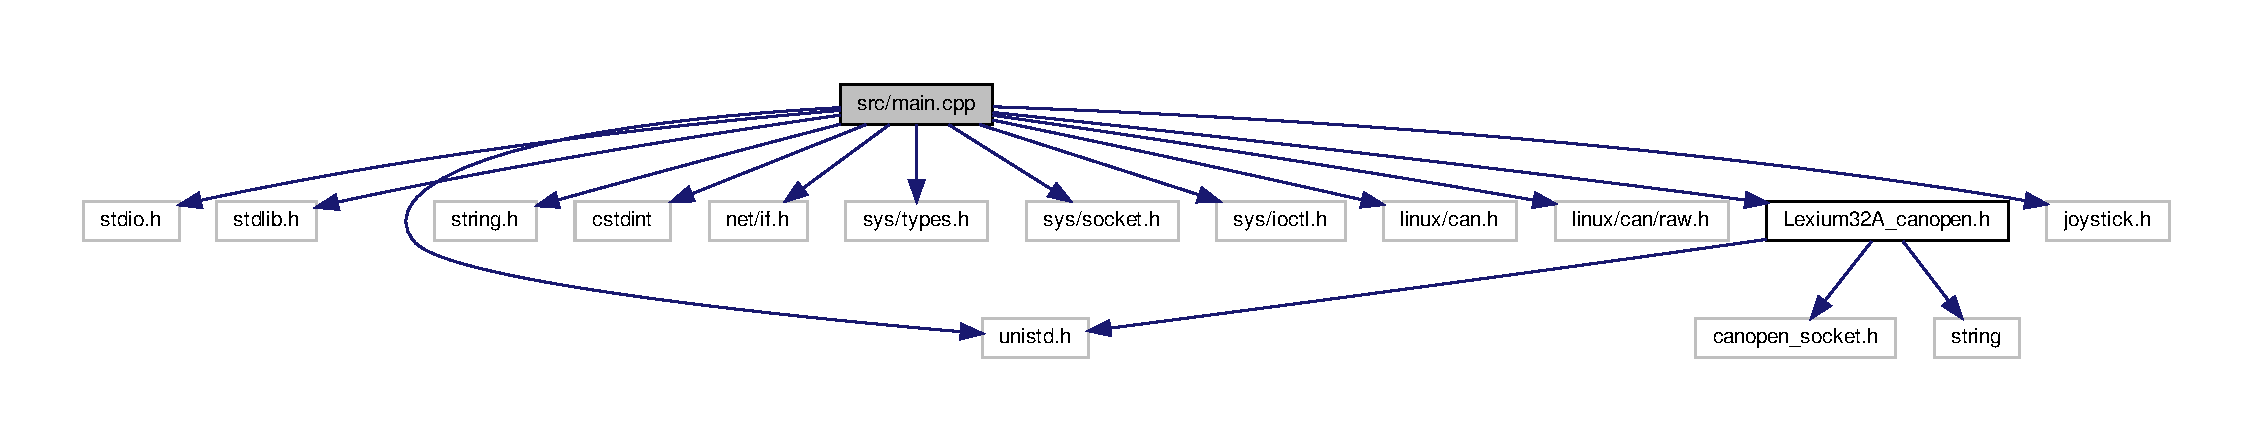
\includegraphics[width=350pt]{main_8cpp__incl}
\end{center}
\end{figure}
\subsection*{Functions}
\begin{DoxyCompactItemize}
\item 
int \hyperlink{main_8cpp_a3c04138a5bfe5d72780bb7e82a18e627}{main} (int argc, char $\ast$$\ast$argv)
\end{DoxyCompactItemize}


\subsection{Function Documentation}
\mbox{\Hypertarget{main_8cpp_a3c04138a5bfe5d72780bb7e82a18e627}\label{main_8cpp_a3c04138a5bfe5d72780bb7e82a18e627}} 
\index{main.\+cpp@{main.\+cpp}!main@{main}}
\index{main@{main}!main.\+cpp@{main.\+cpp}}
\subsubsection{\texorpdfstring{main()}{main()}}
{\footnotesize\ttfamily int main (\begin{DoxyParamCaption}\item[{int}]{argc,  }\item[{char $\ast$$\ast$}]{argv }\end{DoxyParamCaption})}



Definition at line 22 of file main.\+cpp.


%--- End generated contents ---

% Index
\backmatter
\newpage
\phantomsection
\clearemptydoublepage
\addcontentsline{toc}{chapter}{Index}
\printindex

\end{document}
